% Please use the skeleton file you have received in the
% invitation-to-submit email, where your data are already
% filled in. Otherwise please make sure you insert your
% data according to the instructions in PoSauthmanual.pdf
\documentclass[a4paper]{PoS}
\usepackage{subfigure}

\title{Study of Jet Substructure Variables with the SiFCC Detector at 100 TeV}

\ShortTitle{Study of Jet Substructure Variables with the SiFCC Detector at 100 TeV}

\author{\speaker{Chih-Hsiang Yeh}$^a$,S.V. Chekanov$^b$ ,A.V. Kotwal$^{c}$,S. Sen$^{c}$,N.V. Tran$^{b}$,J. Proudfoot$^{b}$,S.-S Yu$^{a}$\\     
     \llap{$^a$}Department of Physics, National Central University\\
     Chung-Li, Taoyuan City 32001, Taiwan\\
     \llap{$^b$}HEP Division, Argonne National Laboratory\\
     9700 S. Cass Avenue, Argonne, IL 60439, USA\\
     \llap{$^c$}Department of Physics, Duke University\\
     Durham, NC 27708, USA\\
     \llap{$^d$}Fermi National Accelerator Laboratory\\
     Batavia, IL 6051, USA\\
     E-mail:  \email{a9510130375@gmail.com},\email{chekanov@anl.gov},\email{kotwal@phy.duke.edu},
     \email{sourav.sen@duke.edu},\email{ntran@fnal.gov},\email{proudfoot@anl.gov},\email{syu@phy.ncu.edu.tw}}

\abstract{We study the performance of jet substructure variables with a detector designed for very high energy proton collisions, the SiFCC detector.  The two-prong jets from Z'$\rightarrow$$WW$ and three-prong jets from Z'$\rightarrow$$t\bar{t}$ are compared with the background from light quark jets at 5, 10, 20 and 40 TeV center-of-mass energies.  The calorimeter geometry is benchmarked in various configurations in order to understand the impact of granularity on variables such as groomed jet mass, Njettiness and energy correlations within the jets. We present results on signal efficiency and background rejection using full GEANT simulations.}

\FullConference{The 39th International Conference on High Energy Physics (ICHEP2018)\\
		4-11 July, 2018\\
		Seoul, Korea}


\begin{document}

\section{Introduction}
In our study, we simulated the Z' bosons with the center-of-mass energies (c.m.) at 5, 10, 20, 40 TeV, and they are forced to decay to two light-flavor jets ($q\bar{q}$) as background, $W W$ or $t\bar{t}$ as signal, where $W$($\rightarrow$$q\bar{q}$) and $t$($ \rightarrow  W^+\>b \rightarrow q\bar{q} b$) decay hadronically. We use different configurations of calorimeter geometry to see whether the smallest configuration can give the best separation power to distinguish signal from background in different jet substructures. We draw the receiver operating characteristic (ROC) curves to quantify the detector performance and find out the cell size that can give the best separation power.

\section{Results and conclusion}
We use soft drop declustering\cite{Larkoski:2014wba} to study the performance of detector with various detector cell sizes and c.m. energies. Figure\ref{1}(a) shows the representative ROC curves for three detector cell sizes at 20TeV with $\beta=0$. For $\beta=0$, the smallest detector cell size, $1~\mathrm{cm}\times1~\mathrm{cm}$, has the best separation power at $\sqrt{s}=$5, 10, and 20 TeV when the signal is $Z' \rightarrow WW$ and at $\sqrt{s}=$10 and 20 TeV when the signal is $Z' \rightarrow t\bar{\mathrm{t}}$. For $\beta=2$, the smallest detector cell size does not have improvements in the separation power with respect to those with larger cell sizes.

We also use several jet substructure variables, including $N$-subjettiness\cite{Thaler:2010tr} and energy correlation function\cite{Larkoski:2013eya} to study. The signals considered are $Z'\rightarrow WW$ ($\tau_{21}$,$C_2^1$) and $Z' \rightarrow t\bar{t}$ ($\tau_{32}$). Figure\ref{1}(b) shows the representative ROC curves for three detector cell sizes at 20TeV with $\tau_{21}$. For all of them, the smallest detector cell size ($1\times1~\mathrm{cm}^2$) does not have the best separation power. It is interesting to note that at very large c.m. energies, the large detector cell sizes have a better separation power than the smallest cell size in most of cases. 

\begin{figure}
\begin{center}
 \subfigure[Soft drop mass with $\beta=0$ and 20 TeV] {
 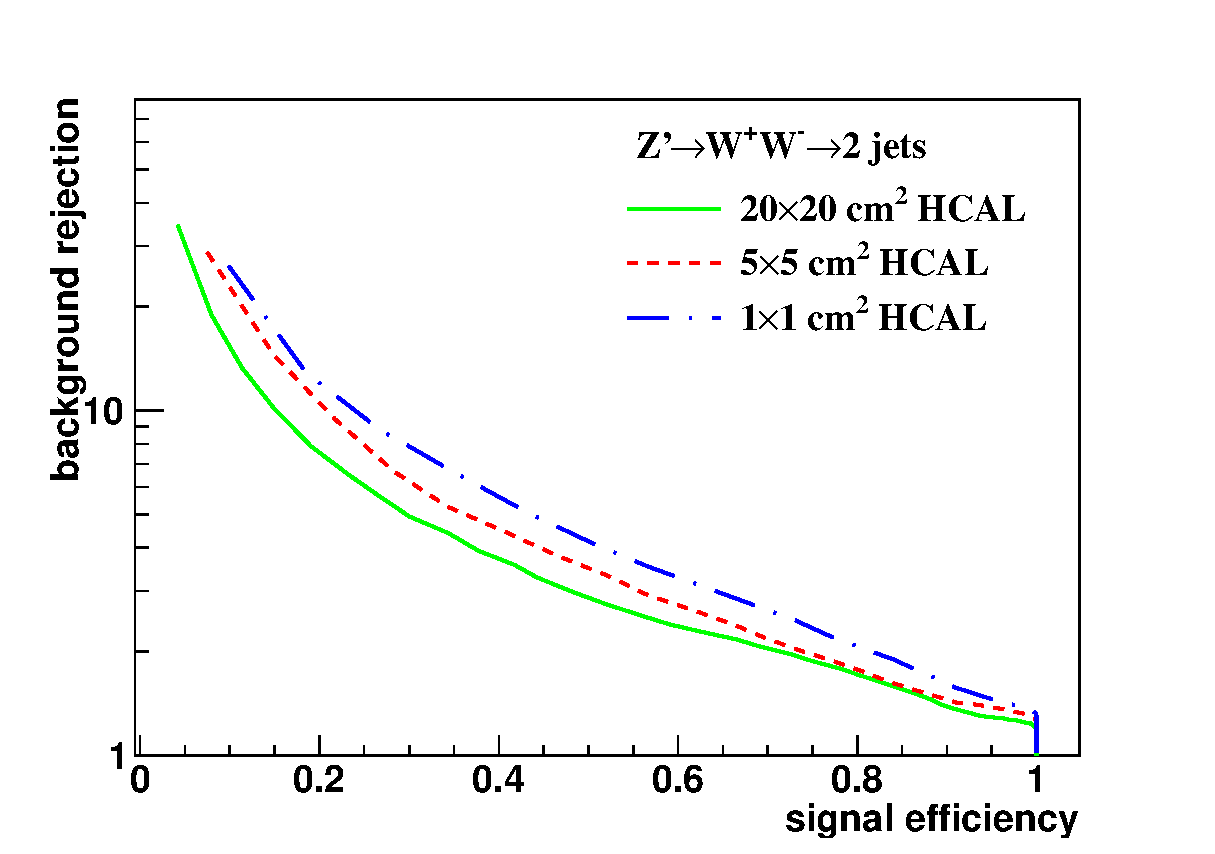
\includegraphics[width=0.4\textwidth]{A_Cluster_mass_mmdt_20tev_eff_1_central_fix_at_Median_bin_ww_qq_log_no_UOF.eps}
 }
 \subfigure[$\tau_{21}$ with 20 TeV] {
 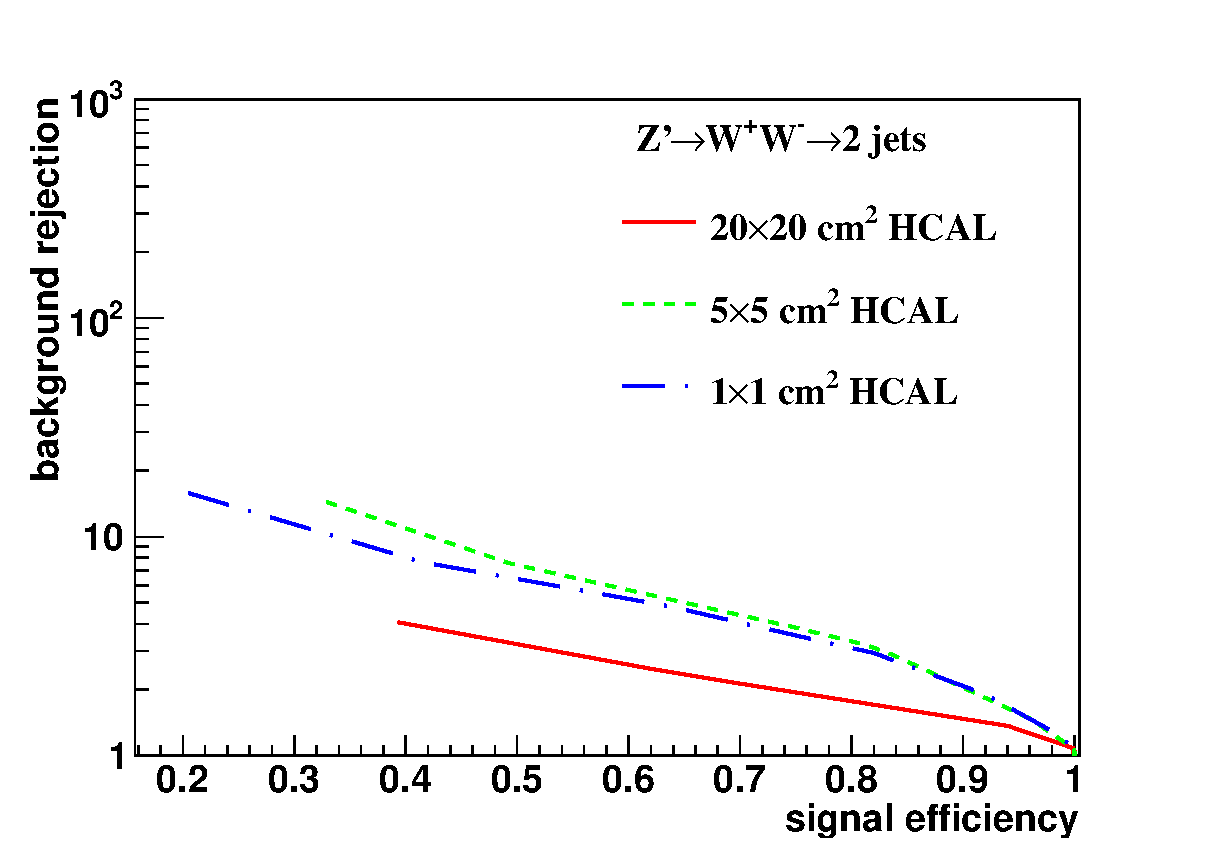
\includegraphics[width=0.4\textwidth]{Rawhit_05GeV_tau21_20tev_eff_1_New2_after_cut_25bins_no_UOF_new_75pa.eps}
 }
\end{center}
\caption{The representative pictures of ROC curves with different jet substructure variables and energies.}
\label{1}
\end{figure}

\begin{thebibliography}{99}
\bibitem{Larkoski:2014wba} 
  A.~J.~Larkoski, S.~Marzani, G.~Soyez and J.~Thaler,
  %``Soft Drop,''
  JHEP {\bf 1405}, 146 (2014)
  doi:10.1007/JHEP05(2014)146
  [arXiv:1402.2657 [hep-ph]].
  %%CITATION = doi:10.1007/JHEP05(2014)146;%%
  %294 citations counted in INSPIRE as of 11 Nov 2018
\bibitem{Thaler:2010tr} 
  J.~Thaler and K.~Van Tilburg,
  %``Identifying Boosted Objects with N-subjettiness,''
  JHEP {\bf 1103}, 015 (2011)
  doi:10.1007/JHEP03(2011)015
  [arXiv:1011.2268 [hep-ph]].
  %%CITATION = doi:10.1007/JHEP03(2011)015;%%
  %467 citations counted in INSPIRE as of 11 Nov 2018
%\cite{Larkoski:2013eya}
\bibitem{Larkoski:2013eya} 
  A.~J.~Larkoski, G.~P.~Salam and J.~Thaler,
  %``Energy Correlation Functions for Jet Substructure,''
  JHEP {\bf 1306}, 108 (2013)
  doi:10.1007/JHEP06(2013)108
  [arXiv:1305.0007 [hep-ph]].
  %%CITATION = doi:10.1007/JHEP06(2013)108;%%
  %167 citations counted in INSPIRE as of 11 Nov 2018
%\cite{Larkoski:2014wba}
\end{thebibliography}

\end{document}
